\newpage

\section{Metode og Proces}
I nedstående afsnit fremlægges metoder og processer brugt til udviklingen af
Dungeons and Gnoblins spillet.

\subsection{Udviklingsforløb}
Projektets endelige mål har været implementeringen af et text-based adventure game.
Hertil har gruppen gjort brug af agile processen til at imødekomme dette mål.

Først har gruppen specifiseret Kravspecifikationerne for spillet, med ønsker om
hvilke features spillet har skulle inkludere. Continuous integration er dernæst
været et vigtigt værktøj til implementeringen af de ønskede features, med et klart
ønske om at integrere nye features ind i projektet få tidligt som muligt.\\

Ugentlig har gruppen været engageret i et SCRUM møde, hvori hvert medlem har infomeret
resten af gruppen om hvor langt i processen de er på daværende tidspunkt. Således har
alle i gruppen altid været klar over projektets fremskridt og evt.\ problemmer der måtte
være opstået i projektet.

\begin{figure}[H]
  \centering
  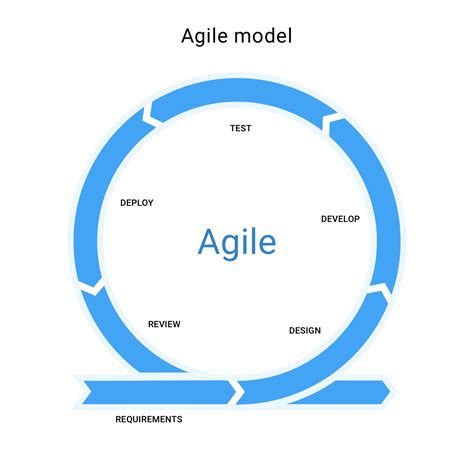
\includegraphics[scale=.5]{02-Body/Images/Agile.png}
  \caption{Viser et billed af agile modellen som består af mangle iterationer
           af design, develop, test, og deploy. Dette minder om continuous integration
           og har hindret mange problemmer for udviklingsforløbet}
  \label{fig:Agile}
\end{figure}

SCRUM og AGILE bringer klarhed til medlemmerne om deres roller og opgaver over en 
kommende tidperiode med en backlog over opgaver, som skal færdiggøres over et sprint (1 uge).
Ugentlige opdateringer og møder omkring potentielle problemmer udviklingsforløbet betyder
at gruppen har kunne tage hånd om evt. problemmer tidligt i forløbet og derved løse dem
før de har udviklet sig til større problemmer.

\newpage

\subsection{Modellering}
Projektet benytter UML til at beskrive og modellere software-- arkitektur
og design, hvilket gør det nemt at simplificere og visualisere strukturen på software
løsningen. 

Selve arkitekturen er vist med C4 modellen som giver et lageret indblik i både
akitekturen på et højt niveau, men med evnen til at give en detaljeret beskrivelse
af systemmets komponenter og deres kommunikation med hinanden.

\begin{figure}[H]
  \centering
  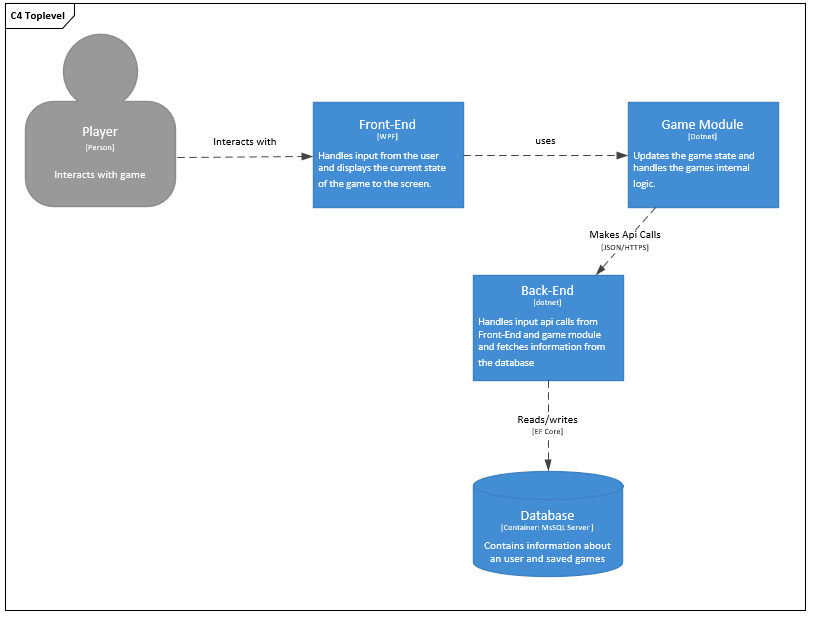
\includegraphics[scale=0.8]{02-Body/Images/C4TopLvlDB.PNG}
  \caption{}
  \label{fig:c4}
\end{figure}

STM og SD diagrammer er brugt til at give programmets udførsel struktur, og fungere
som en hjælp til at visualisere programmets forskellige states og flow of execution.

\subsubsection{Iterativ Udviklingsforløb}

AGILE og continuous integration fungere på en naturlig iterativ måde, der tillader 
ændringer til måde designet og implementeringen undervejs i udviklingsforløbet.
Under hvert SCRUM møde er der taget stilling til om, der skulle laves ændringer i 
gruppens tilgang til projektet, altså om en implementering skulle ændres. \\

Et eksempel har været kommunikationen mellem Game Engine og Frontend, hvor frontend
har haft svært ved at håndtere komplicered return types. Der er sålede lavet
ændringer for at gøre det nemmere for frontend at udnytte den infomation som Game Engine
har returneret efter et funktionskald.

Denne flexible arbejdsmetode har igen ført til at problemmer ikke har kunne vokse men
at der blevet taget hånd om dem mens det stadig har været muligt at håndtere dem.
